\subsection{Überprüfungsmethoden}
\label{methoden}


Man unterscheidet generell zwischen aktiven und passiven Checks.

\subsubsection{Aktive Checks}
asdaasdadasdasdads
asdasd


asdasdas
\subsubsection{Passive Checks}
asdasdasdasdas


Nagios bietet verschiedene Möglichkeiten an solche Dienste zu überprüfen:

\begin{figure}[ht]
	\centering
	   \fbox{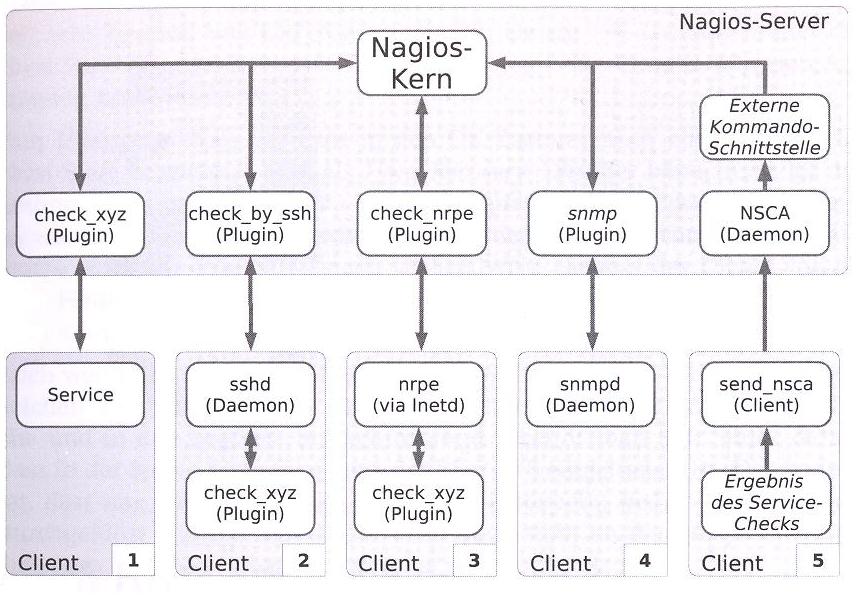
\includegraphics[width=0.95\textwidth]{bilder/nagios-kern.png}}
		\caption[Verschiedene Überwachungsmöglichkeiten von Nagios]{Verschiedene Überwachungsmöglichkeiten von Nagios\protect\footnote}
		\label{nagios-kern}
\end{figure} 
\footnotetext{Quelle: \cite{Barth08} S. 98}


\paragraph{Methode 1 - Netzwerkdienste}

Dienste, die im Netzwerk zur Verfügung stehen (Netzwerkdienste), wie ein Web- oder \gls{FTP}-Server , lassen sich einfach / simpel direkt über das Netz auf ihren Zustand (hin) überprüfen /  testen.
Hierfür muss dem entsprechende Plugin lediglich die Netzwerkadresse mitgeteilt werden, siehe Abbildung \ref{check-http} als beispielhafte Überprüfung eines Webservers.

\begin{figure}[ht]  
	\centering
	   \fbox{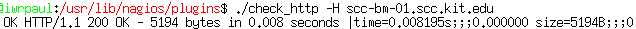
\includegraphics[width=0.85\textwidth]{bilder/check-http.png}}
		\caption{Beispielhafte manuelle Ausführung eines netzwerkbasierenden Servicechecks / HTTP Server Check}
		\label{check-http}
\end{figure}

Der zuvor gezeigte Test eines netzwerkbasierenden Dienstes wird im obigen Bild mit dem Client-Rechner 1 abgebildet.
%Die Überprüfung von nicht netzwerkbasierenden Diensten soll mit den restlichen Client-Rechnern aufgezeigt werden.
Dies ist die einfachste Überwachungsmethode, da keine zusätzlichen Programme oder aufwändige Konfiguration benötigt wird.
Vorteilhaft ist auch, dass der Dienst über das Netzwerk getestet wird, so wie der Benutzer auch auf den Dienst zugreift.
Damit können auch gleichzeitig andere Knotenpunkte wie Switches überwacht werden.

\paragraph{Methode 2 - SSH}

Falls es sich beim Client um ein Unixderivat handelt, ist der entfernte Zugriff auf diesen Client per SSH\footnote{Durch eine Secure Shell (\gls{SSH}) kann man sich eine verschlüsselte Netzwerkverbindung zum entfernten Rechner aufbauen.}-Dienst möglich.
Dazu muss auf dem Client ein \gls{SSH}-Benutzerkonto angelegt sein, mit dem sich Nagios anmelden kann und die öffentlichen Schlüssel (zwischen Nagios Server und Client) ausgetauscht werden, damit keine passwortabhängige Benutzerauthentifizierung (Eingabe von PW) notwendig ist.
Danach können lokale Ressourcen, wie Festplattenkapazität oder Logdateien mit dem entsprechenden Plugin direkt auf dem entfernten Rechner überwacht werden.
Damit der Client diese Plugins verwenden kann, müssen sich die gewünschten Plugins (auch) auf dem Client (lokal) befinden.
Eine beispielhafte Verwendung mit dem dafür gedachten Nagios Plugin \pictext{check\_by\_ssh} (von dieser Überwachungsmethode) wird in Abbildung \ref{check-ssh} gezeigt.

\begin{figure}[ht]
	\centering
	   \fbox{
\includegraphics[width=0.85\textwidth]{bilder/check_by_ssh.png}}
		\caption{Manuelle Ausführung eines Servicechecks über SSH}
		\label{check-ssh}
\end{figure}

\paragraph{Methode 3 - NRPE}

Eine alternative Möglichkeit solche Dienste auf entfernten Rechnern zu überwachen, ist durch den sogenannten Nagios Remote Plugin Executor (\gls{NRPE}).
Hier muss auf dem Client ein "`Agent"' installiert werden, welcher einen Port öffnet mit dem der Agent mit dem Nagios Server kommuniziert.

\begin{figure}[ht]
	\centering
	   \fbox{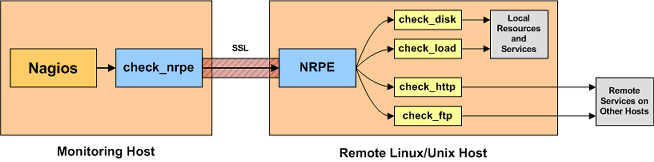
\includegraphics[width=0.9\textwidth]{bilder/nrpe.png}}
		\caption[Aktive Checks mit NRPE]{Aktive Checks mit NRPE\protect\footnote}
		\label{aktivchecks}
\end{figure}
\footnotetext{Quelle: \url{http://www.nagios.org/images/addons/nrpe/nrpe.png}}

Der Nagios Server kann dann Anforderungen über das Nagios-Plugin \pictext{check\_nrpe} an den Client verschicken.
Ein Aufruf dieses Plugins ist dem des \pictext{check\_by\_ssh} Plugins, siehe dazu Abbildung \ref{check-ssh}, sehr ähnlich.

Der Nachteil dieser Variante ist ein zusätzlich geöffneter Port und der höhere / erhöhte Aufwand beim Installieren des Agenten im Gegensatz zum (vermutlich /meistens) bereits laufendem \gls{SSH}-Dienst.\label{sshnrpe}
Zusätzlich gibt es nur die Möglichkeit die Anfragen auf diesem Port auf bestimmte IPs zu beschränken, jedoch nicht den Zugriff durch ein Passwort zu sichern.
Dafür beschränkt sich der \gls{NRPE} (lediglich) auf die auf dem entfernten Client liegenden Nagios Plugins und kann nicht System- bzw. Benutzerkommandos aufrufen, wie bspw. das \pictext{rm} Kommando zum Löschen von Dateien, welche durch den Einsatz von \pictext{check\_by\_ssh} standardmäßig möglich wären.
Sicherheitstechnisch gesehen ist die SSH-Variante kritischer, da es einem Angreifer ermöglicht auf diese System- bzw. Benutzerkommandos zuzugreifen, wenn er die Kontrolle über den Nagios Server erlangt.
Beide Verfahren unterstützen die Verschlüsselung der Datenübertragung zwischen Nagios-Server und Client, so dass keine Informationen im Klartext übertragen werden.

\paragraph{Methode 4 - SNMP}

%nur grob angerissen / kurz / 
Diese Variante wird nur verkürzt behandelt, da sich diese Arbeit hauptsächlich mit der Überwachung von Servern beschäftigt und nicht von Netzwerkkomponenten wie Switches oder Router, die nur durch das Simple Network Management Protocol (\gls{SNMP}) überwacht werden können, wenn mehr Informationen als eine schlichte Erreichbarkeit überprüft / gesammelt werden soll.

Barth schreibt über diese Variante / Überwachungsmethode:
\begin{quote}"`Mit dem Simple Network Management Protocol \gls{SNMP} lassen sich ebenfalls lokale Ressourcen übers Netz abfragen [...]. Ist auf dem Zielhost ein \gls{SNMP}-Daemon installiert [...] kann Nagios ihn nutzen, um lokale Ressourcen wie Prozesse, Festplatten oder Interface-Auslastung abzufragen."' \begin{flushright}\cite{Barth08} S. 101\end{flushright}\end{quote} 

Durch \gls{SNMP} kann auf die strukturierte Datenhaltung der \gls{MIB}\footnote{Die Management Information Base (\gls{MIB}) dient als \gls{SNMP}-Informationstruktur und besteht aus einem hierarchischen, aus Zahlen aufgebauten Namensraum. Ähnliche Struktur wie andere hierarchische Verzeichnisdiensten wie \gls{DNS} oder \gls{LDAP}. Quelle: \cite{Barth08} S.233} in den entfernten Netzwerkknoten zugegriffen werden.
%###########################
Die \gls{MIB}-Struktur ist folgendermaßen aufgebaut:

\begin{figure}[ht]
	\centering
	   \fbox{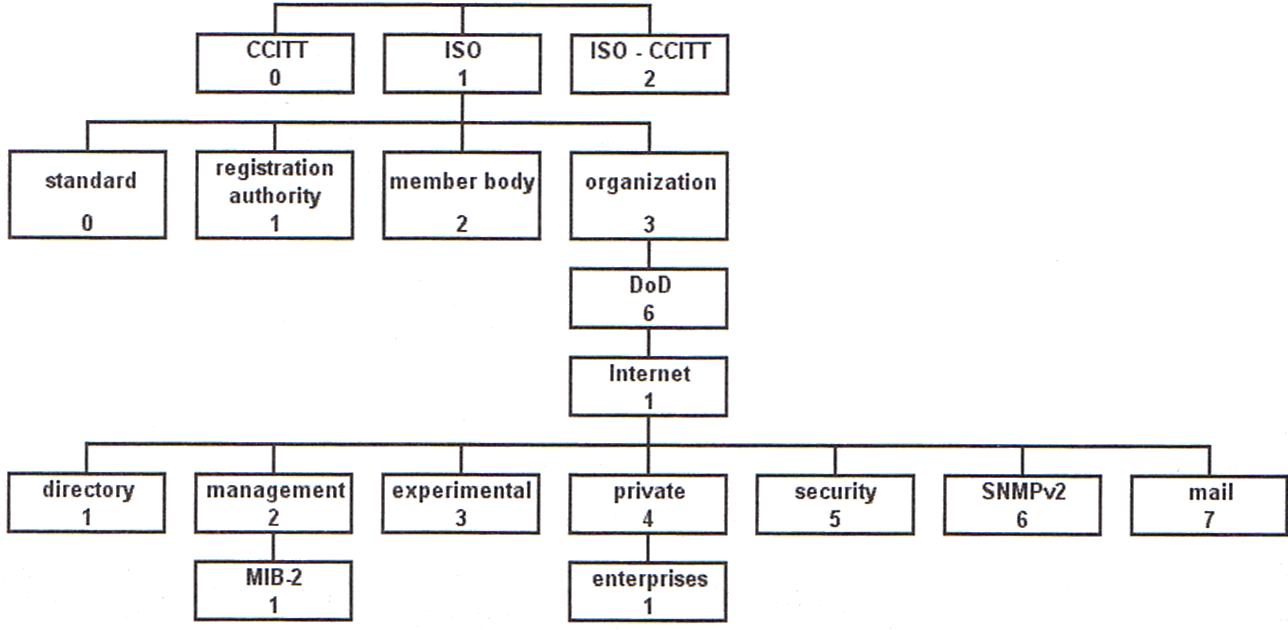
\includegraphics[width=0.95\textwidth]{bilder/mib.png}}
		\caption[Struktur der Management Information Base]{Struktur der Management Information Base\protect\footnotemark}
		\label{munin-mib}
\end{figure}
\footnotetext{Quelle: \cite{Mu08} S. 156}
Anhand dieser Anordnung können die \gls{SNMP}-Plugins von Nagios den gewünschten Wert über das Netzwerk abfragen.
Bei einem Switch werden die auslesbaren Informationen vom Hersteller bestimmt.
Wenn auf einem Rechner eigene Ergebnisse in der \gls{MIB} abgespeichert werden sollen, muss dies durch einen \gls{SNMP}-Daemon eingetragen werden.
Dessen Konfiguration ist im Vergleich zu den anderen Überwachungsmethoden deutlich komplexer.

Es gibt zwei verschiendene Möglichkeiten Dienste mit \gls{SNMP} zu überwachen.
Der Server frägt aktiv den Inhalt der entsprechenden \gls{MIB} Einträgen periodisch ab oder der Client sendet asychron seine Statusmeldungen über \gls{SNMP} an den Nagios-Server.
Bei der letzteren passiven Variante spricht man auch von sogenannten \gls{SNMP}-Traps.


\begin{itemize}
\item Warum wird SNMP nicht verwendet?
\item klartextübertragung des PW bis SNMP 2c
\item Schreibrechte können Schaden anrichten
\item Brute Force attacken ausgesetzt
\item Beschränkte Ausgabemögliochkeit / maximale Datengrösse der Ausgabe -> Logüberwachung nur mit Aufwand möglich autarkes Programm von Nöten, dann muss selbst das Ergebniss in die MIB geschrieben werden, damit Nagios darauf Zugriff erlangt -> zu aufwändig im Vergleich mit Agenten
\end{itemize}

%Einen beispielhaften Zugriff auf SNMP-fähige Geräte wird in Abbildung \ref{munin-snmp} gezeigt.

%\begin{figure}[ht]
%	\centering
%	   \fbox{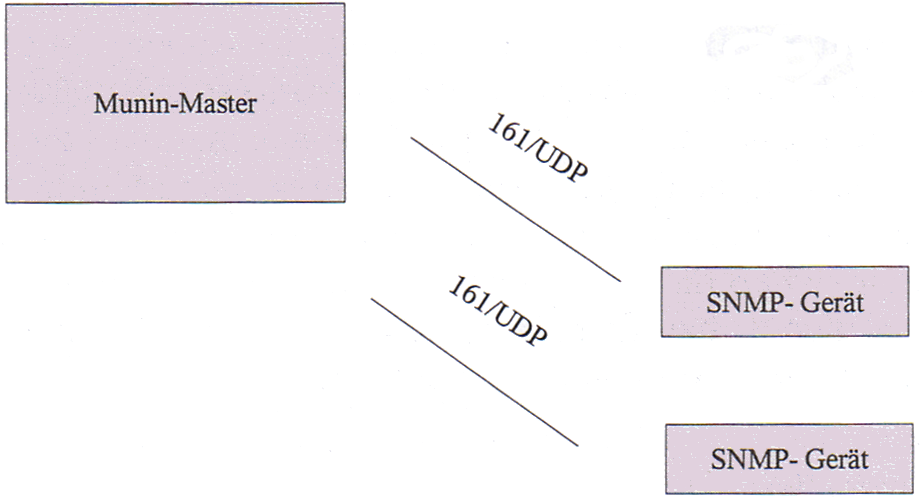
\includegraphics[width=0.5\textwidth]{bilder/snmp.png}}
%		\caption[Beispielhafter Zugriff auf SNMP-fähige Geräte]{Beispielhafter Zugriff auf SNMP-fähige Geräte\protect\footnotemark}
%		\label{munin-snmp}
%\end{figure}
%\footnotetext{Quelle: \cite{Mu08} S. 156}

%##################

\paragraph{Methode 5 - NSCA}
%asynchron!
Diese Methode verwendet passive Checks.
Bei passiven Tests führt der zu überwachende Computer das statuserzeugende Plugin selbst aus und sendet es über ein weiteres Plugin zum Nagios-Server.
Hierfür muss das Testprogramm bzw. Script und das entsprechende Plugin \pictext{send\_ncsa}, welches zum Versenden der Informationen zuständig ist, auf dem Host vorhanden sein.
Auf der anderen Seite muss der \pictext{\gls{NSCA}} (Nagios Service Check Acceptor) auf dem Nagios-Server als Daemon gestartet sein, damit die übermittelten Ergebnisse von Nagios entgegengenommen werden.

Folgende Abbildung soll das Prinzip der passiven Checks verdeutlichen:
%Das Prinzip der passiven Checks lässt sich durch folgende vereinfachte Abbildung
\begin{figure}[ht]
	\centering
	   \fbox{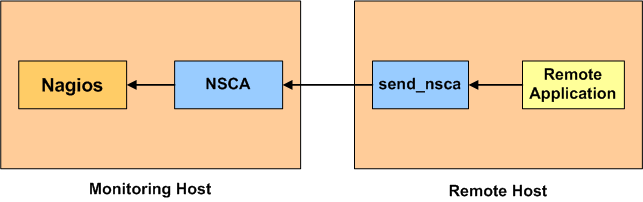
\includegraphics[width=0.9\textwidth]{bilder/nsca.png}}
		\caption[Passive Checks mit NSCA]{Passive Checks mit NSCA\protect\footnote}
		\label{passivchecks}
\end{figure}
\footnotetext{Quelle: \url{http://www.nagios.org/images/addons/nsca/nsca.png}}

Das Testprogramm \textit{Remote Application} wird selbständig vom zu überwachenden Rechner \textit{Remote Host} aufgerufen und übermittelt durch das \pictext{send\_ncsa} Plugin die Ergebnisse über das Netzwerk an den Nagios-Server \textit{Monitoring Host}.
Da auf diesem der NSCA als Daemon läuft können die Ergebnisse an die Nagios-Anwendung zur Auswertung weitergegeben werden.